\section{High-level Architecture}
\subsection{Vixel Proposed Architecture}
Vixel was quite clear on what solution they desired and presented us with a proposed architecture, seen in Figure~\ref{fig:proposed_architecture}. In their proposed architecture the images captured by the camera are sent to a distribution server. From here the video feed is distributed to any connected clients.
In the case where a client user clicks to highlight something on their screen, an interaction request is sent to the host through the distribution server.

\begin{figure}
    \centering
    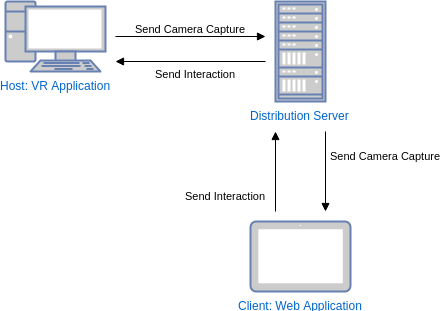
\includegraphics[width=0.8\textwidth]{vixel_stream}
    \caption{Proposed architecture by Vixel}
    \label{fig:proposed_architecture}
\end{figure}

\subsection{Our Architecture}
Our final solution is kept quite close to the original, with some minor differences. As seen in Figure~\ref{fig:our_architecture}, rather than only having one distribution server, two cloud servers are used to achieve the desired functionality. The video stream captured by the camera in the host VR application is sent to a dedicated streaming platform, rather than the distribution server. Interactions between the client and the VR application, such as highlighting, is handled through the Photon Cloud. With the move to dedicated streaming platforms, the client needs a video URL, which is communicated through the Photon Cloud.

\subsubsection{Justification}
Splitting the distribution server into two separate pieces gave us a better focus on combining existing solutions to allow us to finish a functioning proof of concept faster. Having a distribution server would require us to set up a basic streaming platform. It would also need functionality to allow it to speak to both the host side Unity application and the client web application. Such a solution would require us to satisfy potentially complex networking protocols. This was something we neither had time, nor competence to do.

\begin{figure}
    \centering
    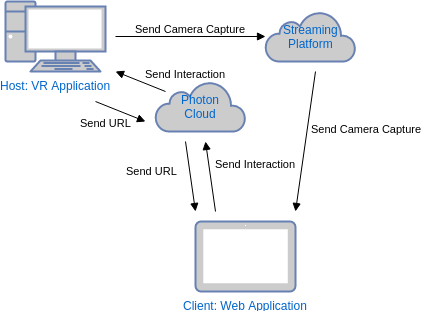
\includegraphics[width=0.8\textwidth]{our_stream}
    \caption{Final Architecture}
    \label{fig:our_architecture}
\end{figure}